%\documentclass[twoside,a4paper,ngerman, german,12pt,authoryear,openright]{book}
%\documentclass[twoside,english,12pt,authoryear,openright]{book}
\documentclass[twoside,12pt,authoryear,openright]{book}

!en \usepackage[english]{babel} 
!de \usepackage[ngerman]{babel} 

\usepackage{geometry} % see geometry.pdf on how to lay out the page. There's lots.
\geometry{a4paper} % or letter or a5paper or ... etc

\usepackage{graphicx}
\usepackage{caption}
\usepackage{subcaption}

% border around all figures
%\usepackage{float}
%\floatstyle{boxed} 
%\restylefloat{figure}

\usepackage{epstopdf}
\usepackage{pslatex}
\usepackage[utf8]{inputenc} 
\usepackage[T1]{fontenc}
\usepackage{a4wide}
\usepackage{fancyhdr}
\usepackage{bookmark}


\usepackage{listings}
\usepackage{courier}
\usepackage{color}
\lstset{
         basicstyle=\scriptsize\ttfamily,         % Standardschrift
%         numbers=left,                           % Ort der Zeilennummern
         numberstyle=\tiny,                       % Stil der Zeilennummern
%         stepnumber=2,                           % Abstand zwischen den Zeilennummern
         numbersep=5pt,                           % Abstand der Nummern zum Text
         tabsize=4,                               % Groesse von Tabs
         extendedchars=true,                      %
%         breaklines=true,                        % Zeilen werden Umgebrochen
%         keywordstyle=\color{blue}\textbf,
         keywordstyle=\ttfamily,
%         frame=tblr,         
 %        keywordstyle=[1]\textbf,                % Stil der Keywords
 %        keywordstyle=[2]\textbf,                %
 %        keywordstyle=[3]\textbf,                %
 %        keywordstyle=[4]\textbf, \sqrt{\sqrt{}} %
%         stringstyle=\color{white}\ttfamily,     % Farbe der String
         showspaces=false,                        % Leerzeichen anzeigen ?
         showtabs=false,                          % Tabs anzeigen ?
         xleftmargin=17pt,
         framextopmargin=17pt,
%         framexleftmargin=17pt,
         framexleftmargin=3pt,
         framexrightmargin=5pt,
         framexbottommargin=4pt,
%         backgroundcolor=\color{lightgray},
         showstringspaces=true                    % Leerzeichen in Strings anzeigen ?        
 }
\lstset{language=C++}

\usepackage{hyperref}

!en \selectlanguage{english}
!de \selectlanguage{ngerman}

\pagestyle{fancy}
\setcounter{secnumdepth}{3}
\setcounter{tocdepth}{3}
\setlength\parskip{\medskipamount}
\setlength\parindent{0pt}

\makeatletter
\makeatother

\newcommand{\at}{\textit{ATmega8}}

\begin{document}
\inputencoding{utf8}

!en \title{Cookbook for Assembly Programming with Arduino and plain 8bit Atmel AVR Micro Controllers}
!de \title{Assemblerkochbuch für Arduino und Atmel AVR Micro Controller}

\author{Felix Morgner and Manfred Morgner}


\maketitle

!en This book is a living piece of work, so if you spot any errors don't hesitate to contact us so we can try to fix them. We are always happy if someone helps us to improve the book, shows us new ways of doing stuff, creates better explanations, throws in faster solutions, cleans up errors ... basically we are happy about everything that helps in the creation of the best cookbook of all time.

!de Dieses Buch ist ein lebendes Werk. Wenn Du Fehler findest kannst Du uns kontaktieren, wir versuchen dann, die Beule auszubeulen. Wir freuen und immer, wenn uns jemand hilft, unser Buch zu verbessern, uns bessere Wege zeigt, verständlichere Beschreibungen demonstriert, schnellere Lösungen einbringt, Fehler beseitigt ... was immer nötig ist um das beste Kochbuch aller Zeiten zu entwickeln.


!en We are going to try to keep the descriptions short while expanding them if requested. This way we can concentrate on the important stuff, we ever that is.

!de Wir werden versuchen, die Beschreibungen kurz zu halten und im Fall von Nachfragen auszubauen. Auf diese Weise können wir uns auf das Wesentliche konzentrieren, was immer das ist.



!en If you want to work along with this book, we suggest getting a copy of the ,ATMEL 8bit AVR instruction set manual':

!de Wenn Du mit diesem Buch arbeiten willst, empfehlen wir mindestens die folgende Dokumentation herunter zu laden ,ATMEL 8bit AVR instruction set manual':

\url{http://www.atmel.com/dyn/resources/prod_documents/doc0856.pdf}



!en We are not going to explain the basics of the instructions used since this would be way beyond the scope of this book and it's already been done in the documentation mentioned above. We are, however, going to explain why we use specific instructions if there are alternatives. Also, we are going to describe specific properties of an instruction if needed.

!de In diesem Buch werden wir die verwendeten Befehle nicht grundlegend erklären. Diese Erläuterungen liegen bereits in der o.g. Dokumentation vor. Natürlich werden wir erläutern wieso wir bestimmte Befehle einsetzen wenn es, im Rahmen des Buches, offensichtliche Alternativen gibt oder bestimmte Spezifika beschreiben sofern es für das Verständnis einer Situation erforderlich ist.



!en This book uses the \at as much as possible to keep the code snippets simple. We don't want to lose ourselves in the specifics of different microcontrollers and we don't want to increase code complexity beyond what's needed.

!de Dieses Buch verwendet für die Umsetzung entweder durchgehend oder überwiegend \at. Diese Einschränkung dient der Vereinfachung der Codebeispiele. Wir wollen und nicht in den Spezifika der Micro Controller Modelle verlieren und unnötig komplexen Quelltext produzieren.



!en One of our goals with this book is, to show what can be achieved with even small microcontrollers. Of course we're aware of the existance of larger and more powerfull devices and that they are readily available for about the same price. However, we believe that it much more impressive to handle a large problem, using a small controller. Take for example the creation of a musical instrument using an \at, some wires and a couple of resistors. Moreover, it can come in pretty handy to know whats at the core, if you're working on a larger project, and assembly-language programms are the core of programming.  

!de Es geht uns auch darum zu zeigen, was bereits mit kleinen Micro Controllern erreicht werden kann. Es ist uns klar, dass grössere, schnellere Micro Controller für ähnliche Preise angeboten werden. Wir sind allerdings der Meinung, dass es viel eindrücklicher ist, mit einem sehr kleinen Micro Controller eine überraschend grosse Aufgabe zu lösen, wie zum Beispiel ein Musikinstrument aus einem \at ein paar Drähten und ein paar Widerständen. Darüber hinaus ist es auch in grösseren Projekten mit umfangreicheren Ressourcen hilfreich zu wissen, worauf es im Kern der Sache ankommt. Und Assemblerprogramme sind notgedrungen in jedem Fall der Kern der Programmierung.



!en This book is all about assembly programming. We don't believe that assembly programms will save the world, even if it's easier to save the world if you are programming in assembly ;-). Every programming language has it's reasons and some of them are even sensible. As a reader of this book, you wan't to learn assembly programming by examples and you like to experiment with real hardware. We try to serve this group of readers by keeping the circuits simple and the cost low.

!de Dieses Buch dreht sich um Assemblerprogrammierung. Wir glauben nicht, das Assemblerprogramme die Welt retten werden. Auch wenn es einfacher ist, die Welt zu retten wenn man in Assembler programmiert ;-). Jede Programmiersprache hat ihren Zweck und manche sind sogar sinnvoll. Der Leser dieses Buches möchte Assemblerprogrammierung anhand von Beispielen erlernen und experimentiert gern mit echter Hardware. Wir versuchen diese Lesergruppe zu bedienen indem wir versuchen, die Schaltungen einfach zu halten und die Kosten dafür niedrig.

\tableofcontents{}
\listoffigures{}
\listoftables{}


!en \part{Simple Samples}
!de \part{Einfache Beispiele}


!en \chapter{Light}
!de \chapter{Licht}



!en X

!de In diesem Kapitel demonstrieren wir die Grundlagen der Assemblerprogrammierung mit AVR Micro Controllern. In den Beispielen werden wir nur das Mindeste an Hardware verwenden. Für die ersten Beispiele benötigen wir lediglich ein Stück Draht und einen mit Strom versorgten Arduino Uno.


\begin{figure}[htbp]
  \centering
  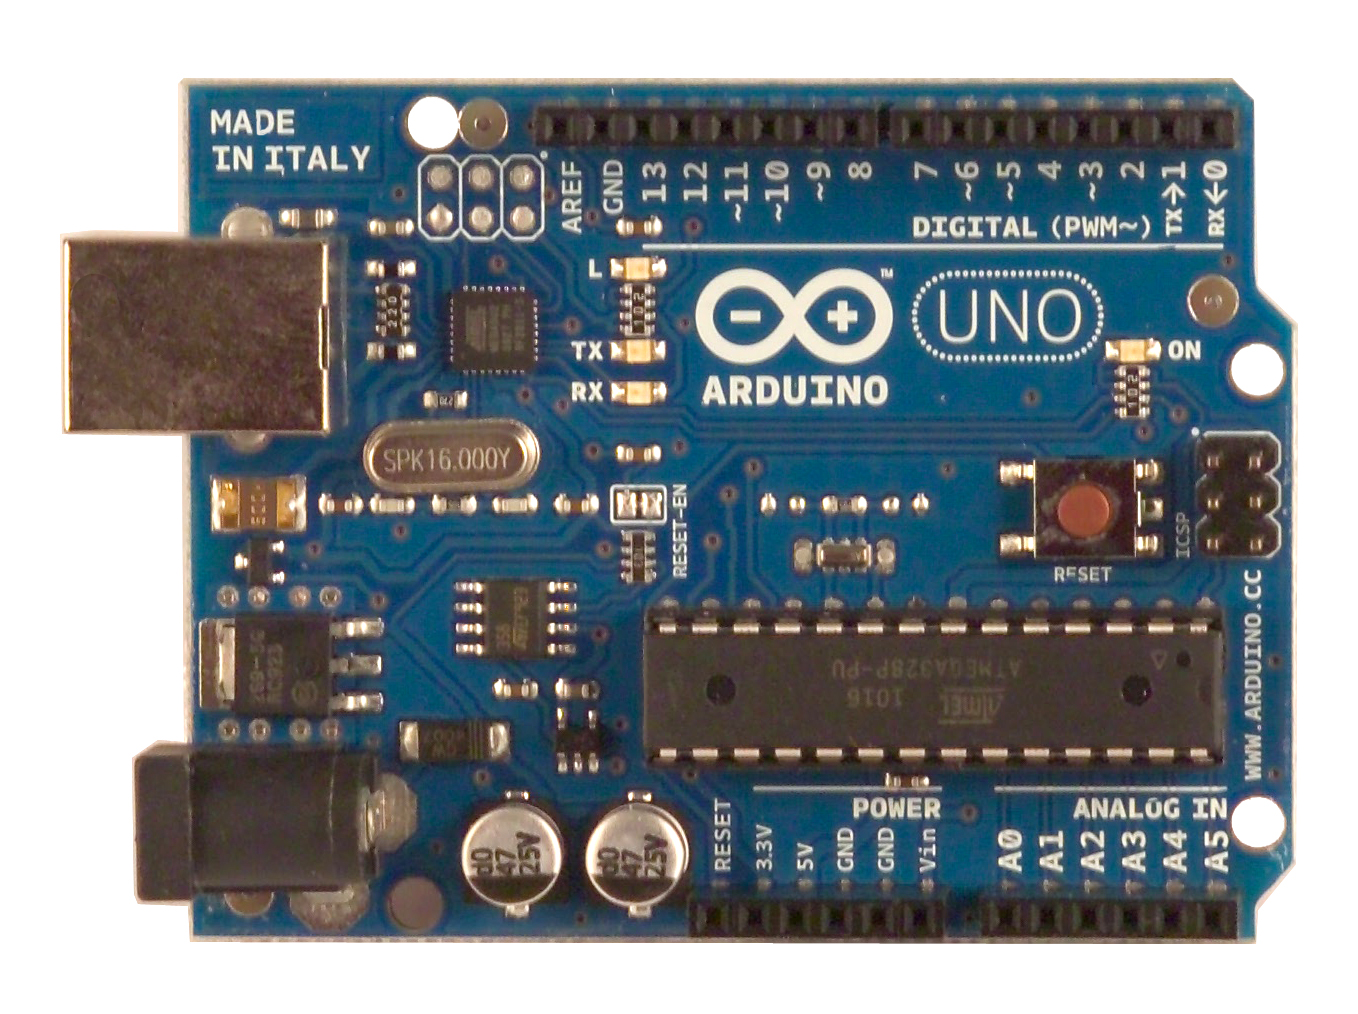
\includegraphics[width=120mm]{Media/www-arduino-cc_ArduinoUnoFront.jpeg}
  \caption{Arduino Uno}
  \label{ArduinoUnoFront}
\end{figure}


\begin{figure}[htbp]
  \centering
  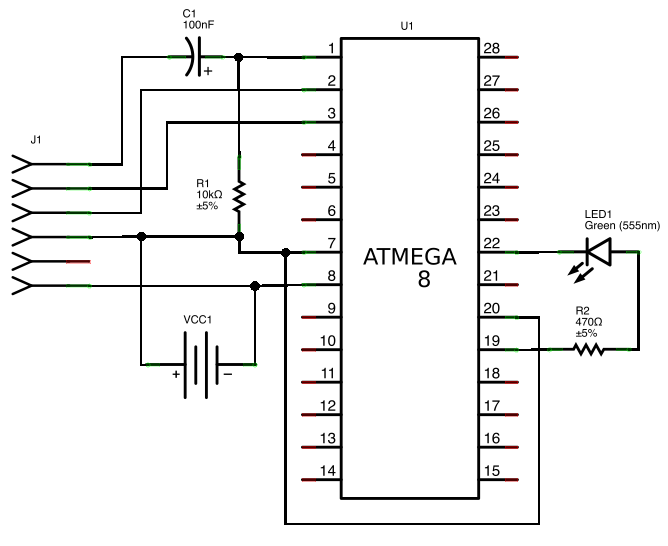
\includegraphics[width=120mm]{LED/S000_let-there-be-light/schema_circuit.png}
!en  \caption{Light - Schema}
!de  \caption{'Licht' Schaltplan}
  \label{atmega8-let-there-be-light-schema}
\end{figure}



!en X

!de Du kannst auch Deine eigene Schaltung aufbauen, wie in Abbildung \ref{atmega8-get-me-on-get-me-off-schema} auf Seite \pageref{atmega8-get-me-on-get-me-off-schema} gezeigt. Das Breadboard Layout kannst Du der Datei \texttt{LED/S000\_LED-Basic-Circuit.fz} entnehmen, eine Fritzing-Datei.



!en X

!de Wir konzentrieren uns darauf, nach Möglichkeit 'Freie und Open Source Software' zu verwenden. Aller Programmcode, den wir hier zeigen ist Freie Software. Das Buch und alles darin ist so frei wie es uns erlaubt wird es zu machen.



!en X

!de Ausserdem versuchen wir zu vermeiden 'Dinge' zu verwenden, die nicht frei sind. Wir möchten niemanden zwingen unfreie Produkte zu benutzen nur um diesem Buch zu folgen. Eins unserer wichtigeren Ziele ist ein Beitrag zur grossen Welt des 'Freien Denkens', der 'Libre Software' und der Zusammenarbeit.



!en \section{Let there be light!}
!de \section{Es werde Licht!}

!en X

!de Das erste Beispiel in diesem Kapitel ist das kleinste Programm, das wir uns vorstellen können, das tatsächlich auch etwas sichtbares tut. Es wird die LED am Arduino Anschluss 13 einschalten.



!en X

!de In Assembler Programmieren heisst, die Macht zu haben! Doch wie wir wissen, erfordert Macht Wissen und Verantwortungsbewusstsein. Jemand der Micro Controller in Assembler programmiert, hat die absolute Macht über den Micro Controller, ob er es will oder nicht! Demzufolge ist ein Mindestmass an Fachwissen erforderlich um verantwortungsbewusst zu handeln. Da es unmöglich ist, von Anfang an gleich alles zu wissen, tastender uns vorsichtig vorwärts. Es gibt aber keinen Grund nicht beliebig im Buch vorwärts und Rückwärts zu blättern. Wir versuchen, die einzelnen Rezepte so unabhängig wie möglich und dennoch aufeinander aufbauend zu gestalten.



!en X

!de Als erstes müssen wir wissen, was der \textit{Digital Pin 13} am Arduino in Wirklichkeit ist. Infolge des Arduinodesigns ist Anschluss 13 am Arduino nicht Bein 13 am \at{}. Das tatsächliche Bein am \at{} zu kennen ist erforderlich um mit dem blanken Chip zu arbeiten. Darüber hinaus ist es erforderlich zu wissen, wie dieser Anschluss im Micro Controller adressiert werden muss. Um das alles heraus zu finden gibt es ein sehr schönes Schaubild: \url{http://www.arduino.cc/hu/Hacking/PinMapping}


\begin{figure}[htbp]
  \centering
  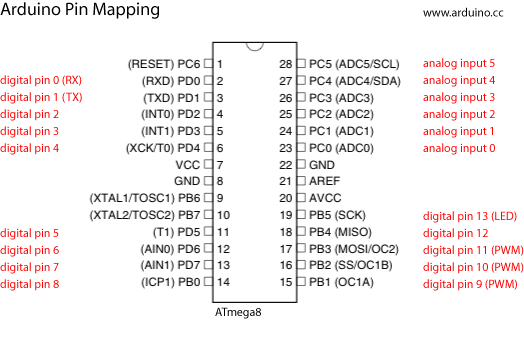
\includegraphics[width=120mm]{Media/www-arduino-cc_Arduino-To-Atmega8-Pins.png}
!en   \caption{Arduino to \at  pins}
!de   \caption{Arduino zu \at  Anschlusszuordnung}
  \label{arduino-to-atmega-pins}
\end{figure}



!en X

!de Nachdem wir zunächst vermutlich genug wissen um verantwortungsvoll zu handeln, programmieren wir unser 8 Byte grosses Programm, dass die LED am 'Adruino Digital Pin 13' erleuchtet.



\begin{lstlisting}
; LED/S000_let-there-be-light.asm

.DEVICE atmega8

.org 0x0000
            rjmp    start 

start:
            sbi     DDRB,         5
            sbi     PORTB,        5
            
main:
            rjmp    main
\end{lstlisting}


!en X

!de So einfach dieses Programm sein mag, es gibt doch ein paar Kleinigkeiten zu beleuchten.



!en X

!de Zunächst müssen wir angeben, welchen konkreten Micro Controller wir verwenden. Das ist erforderlich weil die verschiedenen Modelle verschiedene Adressen für ihre adressierbaren Elemente aufweisen. Dem Assembler wird auf diese Weise mitgeteilt, welche Werte er für welche Elemente verwenden muss. In unserem Beispiel für DDRB und PORTB. DDRB und PORTB sind Platzhalter oder auch 'logische Namen' für Zahlen. Welche Zahlen verwendet werden, entscheidet die Angabe des Micro Controllers hinter \texttt{.DEVICE}. Das geschieht durch:

\begin{lstlisting}
.DEVICE atmega8
\end{lstlisting}



!en X

!de Als nächstes müssen wir den Anfang der Welt benennen. Der Witz hierbei ist, dass wir die volle Wahrheit nie wirklich erfahren! Wir verwenden Symbole um mit dieser Anforderung umzugehen. Wie bereits beschrieben, haben verschiedene Micro Controller verschiedene innere Werte. Aber nicht nur das. Wo exakt sich unser Programm am Ende tatsächlich befinden wird, ist eine kaum beantwortbare Frage. Später werden wir nochmals darauf zurück kommen.


!en X:

!de Da wir also zur Verwendung von Symbolen gezwungen sind, werden wir dementsprechend handeln. Wir werden mit einem Symbol den Startpunkt unseres Programms markieren. Dieses Symbol werden wir 'start' nennen. Was immer auch unser Programm starten wird, es muss diesen Startpunkt kennen:

\begin{lstlisting}
.org 0x0000
            rjmp     start 
\end{lstlisting}



!en X

!de Mit '\texttt{.org}' (Bitte den Punkt am Anfang nicht vergessen!) eröffnen wir eine Liste von Befehlen, die an der bezeichnete Position (hier 0x0000) beginnt. Diese Liste, die auch Tabelle genannt wird, enthält Aktionen, die für beim Eintreten bestimmter Situationen ausgeführt werden sollen. Typischer Weise handelt es sich um Sprungbefehle. Die Situation, bzw, das Ereignis, dass in dieser Tabelle für unser Programm behandelt werden muss, ist, eben dieses Programm zu starten. Glücklicher Weise findet sich der Eintrag für die Aktion '\textit{Programm starten}'an der ersten Stelle diese Tabelle.


 
!en X

!de Dieses Vorgehen scheint auf den ersten Blich sonderbar. Wieso sollte man als erste Anweisung eines Programms zum Anfang des Programms springen müssen? Wieso nicht gleich das Programm starten? Sobald wir mit der Behandlung von Interrupts beginnen, wird das schnell verständlich werden.



!en X:

!de Für die Neugierigen: Die Adressierung innerhalb dieser Tabelle, ist immer relativ zum Anfang der Tabelle. Die Tabelle befindet sich in Wirklichkeit eher nicht an der Position \texttt{0x0000}, aber darauf müssen wir keine Rücksicht nehmen. Genau genommen betreten wir hier bereits eine Art Traumwelt: Wir wissen nicht wirklich, was passiert. Aber in manchen Fällen, wie hier, müssen wir das auch nicht wissen. Wir müssen uns lediglich bewusst sein, dass wir eben nicht wissen, wo im Speicher unsere Programme zu liegen kommen. Das wird wichtig, wenn Speicherzellen angesprochen werden müssen. So können wir die Adresse, an der unser Programm tatsächlich beginnt nicht kennen. Wir müssen des dem Assembler symbolisch erklären. Und zwar so:

\begin{lstlisting}
start:
\end{lstlisting}



!en X

!de '\texttt{start:}' ist eine Marke, ein 'Label'. In unserem Fall ist es eine Sprungmarke. Sie repräsentiert die Adresse der ersten Speicherstelle nach ihrem Erscheinen. In unserem Fall die Adresse des ersten Befehls unseres Programms. Der Assembler wird diese Adresse relativ adressieren, während sie beim Hochladen des Programms auf den Micro Controller in eine absolute Adresse umgewandelt wird.



!en X

!de Die nächste Sprungarke befindet sich bereits hinter dem eigentlichen Ende unseres Programms. Sie ist der Beginn einer unbedingten unendlichen Schleife. Diese Schleife ist erforderlich, weil der Prozessor (CPU) unseres Micro Controllers (MC) arbeitet, solange er Strom hat. Diese Aussage stimmt nicht, in Wirklichkeit kann man nicht nur die CPU anhalten. Das Anhalten der CPU ist aber bereits ein recht komplizierter Vorgang. Wichtig, aber kompliziert. Darum wollen wir hier so tun als wäre es nicht möglich. Da wir die CPU also (momentan) nicht stoppen können, müssen wir ihr etwas zu tun geben was das Ergebnis unseres Programms nicht beeinträchtigt.



!en 

!de Zwischen '\texttt{start:}' und '\texttt{main:}' befindet sich momentan unser eigentliches Programm. Ich nenne das ein Programm der 'Ersten Form'. Ein solches Programm mag nur begrenzten Nutzen haben, aber es ist ganz sicher nicht völlig sinnlos. Diese 'Erste Form' ist die Basis aller erweiterten Programmformen. Ein solches Programm führt folgende Schritte aus:

\begin{itemize}
!en   \item  starts
!de   \item  startet
!en   \item  does something
!de   \item  tut etwas
!en   \item  loops forever, doing nothing
!de   \item  tritt in eine Endlosschleife, tut nichts mehr
\end{itemize}



!en X

!de Sofern das Programm im inneren der Endlosschleife etwas tut, nenne ich das die 'Zweite Form' eines Programms. Eine 'Dritte Form' darf für später erwartet werden. Sei es wie es sei, unser aktuelles Programm wurde speziell entworfen um einige wichtige Regeln guter MC Programmierung zu demonstrieren.



!en X

!de Die beiden Befehle, die die Aufgabe unseres Programms erfüllen tun das folgende:

\begin{itemize}
!en   \item  declare pin 5 at PORTB as output pin
!de   \item  Bit 5 an PORTB als Ausgabepin festlegen
!en   \item  set pin 5 at PORTB under power to enlighten our LED
!de   \item  Bit 5 an PORTB einschalten um die LED zu erleuchten
\end{itemize}

\begin{lstlisting}
            sbi     DDRB,         5
            sbi     PORTB,        5
\end{lstlisting}

!en X:

!de Am Ende die nicht enden wollende Schleife:

\begin{lstlisting}
main:
            rjmp    main
\end{lstlisting}



!en This is all the program does and there is nothing more about it. You will discover, that this program demonstrates prudence and thrift. 

!de Das ist alles was das Programm tut. Allerdings tut es das mit Bedacht und Sparsamkeit!



!en X:

!de Ein PORT eines 8bit Micro Controllers waltet die 8 Bit eines Bytes in 8 einzelne, unabhängige Beine in der Aussenwelt. An unserem \at{} kann jedes dieser Beine verwendet werden um eine der folgenden Funktionen zu erfüllen:

\begin{itemize}
!en   \item Put a signal to his pin
!de   \item Ein Signal ausgeben
!en   \item Read a signal from its pin which may be +5V or GND as 1 or 0
!de   \item Ein Signal lesen, dass VCC oder GND ist, als Repräsentation für 1 oder 0
!en   \item Read a signal from its pin which may be 'not GND' or GND as 1 or 0
!de   \item Ein Signal lesen, dass 'nicht GND' oder GND ist, als Repräsentation für 1 oder 0
\end{itemize}



!en X

!de Jedes Bein kann unabhängig von jedem anderen Bein konfiguriert werden um eine dieser Operationen auszuführen. Alles am gleichen Port, 8 Bit/Beine mit einem einzigen Byte!



!en X

!de An einigen Beinen sind weitere Funktionen möglich wie

\begin{itemize}
!en   \item power saving modes (the pin becomes deaf)
!de   \item Energiesparmodus (das Bein wird abgeschaltet)
!en   \item PWM modes
!de   \item Pulsbreitenpodulierter Signalgenerator (PWM)
!en   \item analog to digital converting
!de   \item Analog-Digital-Wandlung
!en   \item interrupts
!de   \item Interruptempfang
\end{itemize}



!en X

!de In unserem Programm verwenden wir den Befehl \texttt{sbi} um das Bit 5 anzusteuern anstatt den Befehl \texttt{out} mit dem Parameter \texttt{1 << 5} zu verwenden, was auf den ersten Blick zum gleichen Ergebnis führen würde. Wir wollen aber einzig bit 5 ansteuern! \texttt{out 1 << 5} würde dummer Weise aber nicht nur Bit 5 auf \texttt{1} setzen, sondern gleichzeitig alle anderen Bits, ihrer 7 Stück, auf \texttt{0}!


!en X:

!de Auch wenn wir - für den Augenblick - wissen, dass alle anderen Bits nicht benutzt sind, werden wir bald mit den eher typischen Situationen konfrontiert:

\begin{enumerate}
!en   \item We will become less and less sure about the usage of bits we don't use in a particular situation. Especially if we are developing a library.
!de   \item Wir werden zunehmen unsicher werden, welche Bits/Anschlüsse tatsächlich benutzt werden, während wir etwas bestimmtes programmieren. Auch und besonders wenn wir Bibliotheken verwenden. Dann sowieso nicht!
!en   \item We don't know what happens if we send \texttt{0}'s to pins we don't know.
!de   \item Wir wissen nicht was passiert wenn wir \texttt{0} an Bits senden, die wir momentan gar nicht \textit{betrachten}.
\end{enumerate}



!en X

!de \emph{Ein wichtiges Konzept guten Programmierens ist, so wenig wir irgend möglich zu tun.}



!en If there is nothing to be done, don't do it! Especially in micro controllers where action means energy loss. So if we need to manipulate a bit, we should not manipulate others bits except we have a good reason to do so. Currently we have not.

!de Wenn nichts zu tun ist, dann tu's nicht! Das gilt besonders bei Micro Controllern, wo jede Aktion Energieverbrauch bedeutet. Noch schlimmer: Ein unnötig bewegtes Bit könnte zu destruktiven Aktionen angeschlossener Geräte führen! Wenn wir also ein Bit ansteuern wollen, sollten wir genau ein Bit ansteuern und nicht mehr, ausser wir haben gute Gründe, diese Regel nicht zu beachten. Momentan haben wir keine.



!en X

!de Wir wollen nicht Beine Aufwecken, die auch auch in Ruhe schlafen könnten. Denn möglicher Weise würden diese Anschlüsse alle zur Verfügung stehende Energie verheizen, im Sinn von heizen!

!en \section{Get me on, leave me off}
!de \section{Mach' mich an, lass' mich aus}

!en X

!de Zuerst die erweiterte Schaltung

\begin{figure}[htbp]
  \centering
  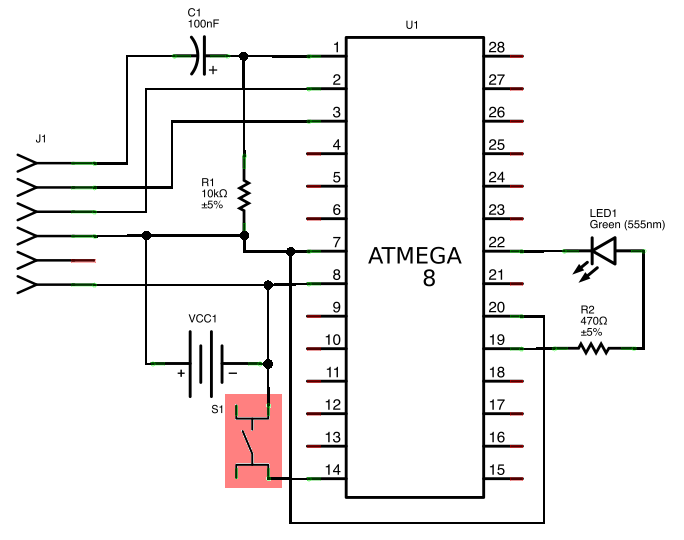
\includegraphics[width=120mm]{LED/S002_get-me-on-get-me-off_Circuit_schema.png}
!en   \caption{Get me on, get me off - Schema}
!de   \caption{Mach' mich an, lass' mich aus - Schaltplan}
  \label{atmega8-get-me-on-get-me-off-schema}
  \label{atmega8-get-me-on-get-me-off-schema}
\end{figure}


!en Second the code

!de Anschliessend das Programm


\begin{lstlisting}
; LED/S002_get-me-on-get-me-off.asm

.DEVICE atmega8

.org 0x0000
            rjmp     start

start:
            sbi     DDRB,         5
            cbi     DDRB,         0
            sbi     PORTB,        0

main:
            sbic    PINB,         0 ; 1 cycles if false or 2
            rjmp    led_on          ; 2 cycles
            cbi     PORTB,        5 ; 1 cycle
            rjmp    led_ok          ; 2 cycles
led_on:
            sbi     PORTB,        5 ; 1 cycle
led_ok:
            rjmp    main            ; 2 cycles
\end{lstlisting}

!en X

!de Wie zu vermuten war, handelt es sich hier bereits ein Programm der 'Zweiten Form'. Es tut nicht nur etwas \textit{vor} der Endlosschleife, sondern ebenfalls etwas darin. Dieses Programm hat wirklich viel zu tun, wie noch sehen werden.



!en X

!de Der erste Unterschied zum vorherigen Programm ist, dass wir ein zusätzliches Bein benutzen, diesmal um ein Eingangssignal zu erkennen. Um dieses Bein, Bit 0 an Port B = Bein 14 am MC, auf den Input Modus zu schalten, senden wir eine \texttt{0} an das entsprechende 'Data Direction Register' (\texttt{DDR}), also \texttt{cbi DDRB, 0}. Ausserdem senden wir eine \texttt{1} auf das Bit am entsprechenden Port, \texttt{sbi PORTB, 1}. Was im Ausgabemodus bedeuten würde 'Schalte VCC an das Bein', heisst im Eingabemodus: 'Schalte den pull-up-Widerstand\footnote{Ein pull-up-Widerstand ist ein Widerstand, der dazu benutzt wird, um den Signalpegel an einem Bein 'hoch' (auf VCC) zu legen = \texttt{1}. Er dient dazu um an einem Eingangsbein auch dann einen stabilen Zustand zu erreichen, wenn kein Element angeschlossen ist.} zu'.



!en X

!de Danach können wir vom Eingangsbein den Status 'EIN' oder '1' lesen. Um eine Reaktion am MC zu erreichen und das Eingangssignal auf 'AUS' oder '0' zu setzen, müssen wir das Beim auf GND ziehen.



!en X

!de Wenn wir das machen, schaltet unser Programm das Licht aus solange wir das Eingangsbein auf Masse legen. Das ist nicht direkt eine Anwendung mit der wir gross angeben können. Für uns ist es dennoch grossartig weil wir verstehen was passiert!



!en If you follow the programs flow:

%de Das Programm läuft folgendermassen ab:

\begin{enumerate}
!en   \item Initialise system and all connected devices
!de   \item Initialisiere das System und die angeschlossenen Geräte
!en   \item (*) Read bit 0
!de   \item (*) Lese Bit 0
!en   \item Set bit 5 accordingly
!de   \item Setze Bit 5 entsprechend
!en   \item Continue with (*)
!de   \item Weiter bei (*)
\end{enumerate}



!en X

!de Jemand, der dieses Programm unter dem Blickwinkel der Sparsamkeit betrachtet, wird sich womöglich fragen, wieso ständig das gleiche Signal auf das Ausgabebit ausgegeben wird. Wenn wir einmal grob annehmen, dass unser Programm das Eingangsbit ca. eine Million mal pro Sekunde liest (eher 8 Mio. mal bei 8MHz ), ist einzusehen, dass ein Mensch mit einem Tasten kaum 'Last' für unseren MC erzeugen kann. Wenn ein Mensch auf den Schalter einhämmert so schnell er kann, passiert aus der Sicht des Micro Controllers so gut wir gar nichts, das Signal ändert sich auf diese Weise für den MC in historischen Zeiträumen.


!en X

!de Die tatsächliche Abfragefrequenz ist möglicher Weise unterschiedlich für die beiden Systemzuständen (Signal \texttt{1} oder \texttt{0}). Wir rechnen kurz nach:

\begin{enumerate}
!en   \item X
!de   \item Signal = '\texttt{1}' entspricht 5 Zyklen
!en   \item X
!de   \item Signal = '\texttt{0}' entspricht 7 Zyklen
\end{enumerate}



!en X

!de Die Schleifendurchlauffrequenz können wir einfach berechnen, indem wir die Taktfrequenz des Prozessors durch die Anzahl der erforderlichen Taktzyklen für einen Schleifendurchlauf teilen.

\begin{equation}
f_{Loop} = \frac{f_{CPU}}{d}
\end{equation}

!en X

!de Wobei d die 'Dauer' eines Schleifendurchlaufs in Zyklen pro Schleifendurchlauf ist. Das bedeutet, dass der MC ohne Druck auf den Taster 8/5 Mio. Mal pro Sekunde den Schaltzustand des Tasters anfragt und bei gedrücktem Taster 8/7 Mio. Mal pro Sekunde.


!en X

!de Solche Abfragefrequenzen sind im Allgemeinen unsinnig. Es gibt Fälle, in denen auch die Bedienung von Tasten durch Menschen zeitkritisch sind, wenn es sich um Musikinstrumente handelt, kommt es auf Millisekunden an. Aber um ein Licht einzuschalten, genügen problemlos 30 Schleifendurchläufe je Sekunde. Mehr kann der Mensch ohnehin nicht erkennen. Kann man das System also optimieren? Wir glauben nicht.



!en X

!de Gibt es andere Lösungen? Ja, die gibt es!



!en \subsection{CPU Frequency}
!de \subsection{CPU Frequenz anpassen}

!en X

!de Wir könnten die Taktfrequenz, mit der die CPU operiert senken. Je nach Einsatzfall kann das tatsächlich helfen, Energie zu sparen, wäre aber damit verbunden, die Rechenleistung des Systems zu reduzieren und kann nachteilig wirken, wenn zusätzliche Aufgaben erledigt werden.



!en X

!de Es kann allerdings nicht schaden, sich in jedem Fall Gedanken über die Taktfrequenzen zu machen, die in einem Micro Controller zusammenkommen. Sowohl nach unten wie auch nach oben. Letztlich beeinflusst eine solche Entscheidung auch die Auswahl des Micro Controllers als solchem.



\subsection{Interrupts}

!en X

!de Vielleicht könnte man auch Interrupts verwenden, um die Signalisierung des Schalterstatus umzukehren. Der Mikroprozessor erledigt dann die Abfrage für uns und signalisiert dem Programm aktiv, dass der Knopf gedrückt wurde. Dieses Verfahren macht einen ruhigeren Eindruck, läuft technisch aber auf das gleiche Prinzip hinaus, mit dem Unterschied, dass wir einen grossen Aufwand zur Initialisierung der Interruptauslösung betreiben müssten, ohne dass die CPU weniger rotieren hätte. Die Hauptprogrammschleife wäre dann leer. Doch sie würde sich auch leer mir dem vollen CPU Takt um sich selbst drehen.



!en X

!de Das heisst, das Programm wird komplizierter - wie wir sehen werden schränkt ein solches Verfahren sogar die Anzahl der Pins ein, die als Schaltereingang benutzt werden können - aber die CPU Last bleibt gleich.


!en X

!de Wirklich nützlich wird dieses Verfahren erst, wenn die CPU abgeschaltet werden könnte, während sie auf einen Interrupt wartet oder - dann sowieso - wenn das Programm parallel noch eine Reihe anderer Aufgaben zu lösen hätte. Beides werden wir noch demonstrieren. Beides ist in der aktuellen Phase aber noch zu komplex.



!en \subsection{X}
!de \subsection{Statusverwaltung}



!en X

!de Wir könnten den zuletzt ausgegebenen Status speichern. Dann könnten wir in der nächsten Programmschleife prüfen ob sich der eingelesene Status zum vorherigen Status geändert hat und nur dann ein Signal an das Bein ausgeben, wenn eine solche Änderung vorliegt. Das könnte uns ersparen, 8/5 oder 8/7 Mio. Mal pro Sekunde den unveränderten Status an die LED auszugeben.



!en X

!de Das klingt gut und einfach, ist es aber leider nicht! Es ist nicht nur nicht einfach, es ist gefährlich, kostspielig und kompliziert. Und es ist effektiv sinnlos weil wir eine Menge Aufwand treiben würden, ohne dass sich wirklich etwas verbessert.



!en X

!de Dieses Konzept ist gefährlich weil das Programm aus dem Rhythmus kommen könnte. Danach würde es falsch herum arbeiten oder überhaupt nicht mehr auf Eingangssignale reagieren.



!en X

!de Es ist kostspielig weil das Programm nicht nur viel grösser würde, wir würden ausserdem ein CPU Register verbrauchen (um den Status zu speichern) und wir haben um \at{} total nur 32 Stück von denen nur die Hälfte einfach zu benutzen ist!



!en X

!de Und es ist kompliziert weil wir zwei unabhängige Einheiten im Gleichlauf halten müssen (das Licht und das Statusregister) um vielleicht einen Effekt zu erzielen. Das ist ein grosses Risiko und ein Nachteil gegenüber der vorliegenden Lösung.



!en X

!de Aus diesen Gründen liegen wir vielleicht nicht falsch mit der Vermutung, dass die Entwickler unseres Micro Controllers ihren Chip so entwickelt haben, dass in Wirklichkeit gar nichts gemacht wird, wenn wir eine '1' auf ein Steuerbit senden, dass bereit auf '1' gesetzt ist. Diese Form der Optimierung darf man erwarten.



!en X

!de In der Summe heisst das, dass wir momentan am Ende unsere Möglichkeiten sind Wir müssen hier also bei der vorliegenden Lösung bleiben. Die Vorgeschlagenen Ansätze werden später allerdings noch aktuell werden.
!en \section{Stable Decisions}
!de \section{Stabile Entscheidungen}



!en X

!de In diesem Beispiel sollten wir etwas sinnvolleres unternehmen. Das werden wir unter Beibehaltung des Programmrahmens. Es bleibt also zunächst bei einem Programm der 'zweiten Form': Ein Programm, dass etwas in seiner Endlossschleife tut.



!en X

!de Das Programm speichert einen von zwei Zuständen ;-) und stellte das Licht an oder aus, abhängig vom gespeicherten Zustand. Diese Erklärung ist nicht ganz richtig. Darum versuche ich es noch einmal.



!en X

!de Das Programm erkennt ein Signal am Eingang, an einem Phasenwechsel. Ein vollständiges Signal besteht aus dem Wechsel des Eingangspegels von HOCH nach NIEDRIG und wieder nach HOCH. Das Programm interessiert sich nur für den Wechsel, worauf auch wir uns immer konzentrieren sollten. Wenn der Signalpegel von HOCH nach NIEDRIG wechselt, kehrt unser Programm den Status der LED um. Wenn das Licht AN war, geht es AUS und umgekehrt. 



!en X

!de Das Ausgangssignal wird umgekehrt wenn der Eingangspegel von HOCH nach NIEDRIG wechselt weil durch die Verwendung eines 'pull up' Widerstandes der Pegel am Eingang HOCH ist, während der Knopf \textit{nicht} gedrückt wird. Auf den Wechsel von HOCH nach NIEDRIG zu reagieren bedeutet also, die Aktion in dem Moment auszulösen wenn der Schalter gedrückt wird.



!en X

!de Wir dürfen davon ausgehen, dass das das ist, was der Benutzer des Programms höchstwahrscheinlich erwartet. Denn ein solches Verhalten entspricht den meisten Lichtschaltern mit denen wir konfrontiert werden.



!en X

!de Das \textit{elektrische} Signal, auf das unser MC am gewählten Eingangsbein wartet ist der Wechsel des Spannungszustandes von HOCH (VCC) nach NIEDRIG (GND). Um exakt zu sein sollten wir die Erwartungshaltung so formulieren:

\begin{center}
!en The \emph{Signal} the MC is waiting for is the \emph{Change} form VCC to GND.
!de Das \emph{Signal} auf dass der MC wartet ist der \emph{Wechsel} von VCC nach GND.
\end{center}



!en X

!de Zum ersten Mal (und hoffentlich nicht zu oft) haben wir uns mit einem dynamischen Zustand zu beschäftigen. Wenn der Wechsel des Pegels das Signal ist, müssen wir den Umstand 'hat gewechselt' erkennen. Wenn also der Pegel NIEDRIG erkannt wird, \textit{unmittelbar} nachdem der Pegel HOCH war (also in der nahen Vergangenheit!), haben wir es gewissermassen mit Vergangenheitsbewältigung zu tun. Dafür muss sich unser Programm zum ersten Mal in einem Verarbeitungszyklus an einen vergangenen Pegel/Messwert aus dem vorherigen Verarbeitungszyklus erinnern.


!en X:

!de Und das geht so:

\begin{lstlisting}
; LED/S004_stable-decisions.asm

.DEVICE atmega8

.org 0x0000
            rjmp    start

start:
            sbi     DDRB,         5
            cbi     DDRB,         0
            sbi     PORTB,        0

            ldi     r16,          1

main:
            sbic    PINB,         0
            rjmp    led_keep
            tst     r16
            breq    led_ok
            clr     r16
            sbis    PINB,         5
            rjmp    led_on
            cbi     PORTB,        5
            rjmp    led_ok
led_on:
            sbi     PORTB,        5
            rjmp    led_ok
led_keep:
            ldi     r16,          1
led_ok:
            rjmp    main
\end{lstlisting}



!en X:

!de Wie man leicht erkennen kann, ist dieser Programmcode nicht leicht zu verstehen. Um dieses Missstand abzustellen, wollen wir ein paar symbolische Namen in die Suppe rühren. Die Grundlagen sind:

\begin{itemize}
!en   \item \texttt{.equ} means: 'a name for a value'
!de   \item \texttt{.equ} heisst: 'ein Name für einen Wert' (Zahl oder Text)
!en   \item \texttt{.def} means: 'a name for an entity'
!de   \item \texttt{.def} heisst: 'ein Name für ein Ding' (z.B: CPU Register)
\end{itemize}



!en X

!de \texttt{DDRB} zum Beispiel ist bereits eine Nummer. Diese Nummer ist in einer Datei hinterlegt, die durch die Geräteauswahl bestimmt und geladen wird. In unserem Fall soll \texttt{DDRB}, unabhängig von seinem Wert, unsere Eingangs- und Ausgangsbeine bezeichnen. Wir bilden den Namen aus \texttt{ctl} als Präfix für 'Control Port' und \texttt{IO} als Abkürzung für Input\&Output. Das ergibt \texttt{ctlIO}.



!en X

!de Ein anderes Beispiel: \texttt{bit} für 'Bitnummer' und \texttt{Input} für Inputbit, macht \texttt{bitInput}. Oder \texttt{b} für 'Byte' und \texttt{Status} für 'Statusregister' macht \texttt{bStatus}



!en X

!de Es spricht nichts dagegen, eine eigene Namenskonvention zu entwickeln, eine sinnvolle Struktur sollte sich daraus aber ergeben. So könnte man beispielsweise auch \texttt{InputCtl} verwenden und \texttt{InputBit} usw. Wie es einem am leichtesten Fällt oder wie es einem vorgeschrieben wird.

\begin{lstlisting}
; LED/S005_stable-decisions+symbols.asm

.DEVICE atmega8

.equ ctlIO     = DDRB    ; DDRB  is our I/O control register
.equ prtIO     = PORTB   ; PORTB is our I/O output port register
.equ pinIO     = PINB    ; PINB  is our I/O input pin register

.equ bitOutput = 5       ; bit 5 is our output bit
.equ bitInput  = 0       ; bit 0 is our input bit

.equ FALSE     = 0       ; 0 will be FALSE or OFF
.equ TRUE      = 1       ; 1 will be TRUE  or ON

.def bStatus   = r16     ; the last state will be stored in 'r16'
\end{lstlisting}



!en X

!de Diese Massnahme macht den Code meistens leichter lesbar und somit leichter zu verstehen und zu interpretieren. Jener sieht dann so aus (fast schon wie eine Hochsprache):

\begin{lstlisting}
.org 0x0000
            rjmp    start

start:
            sbi     ctlIO,        bitOutput
            cbi     ctlIO,        bitInput
            sbi     prtIO,        bitInput

            ldi     bStatus,      HIGH

main:
            sbic    pinIO,        bitInput
            rjmp    led_keep
            tst     bStatus
            breq    led_ok
            clr     bStatus
            sbis    pinIO,        bitOutput
            rjmp    led_on
            cbi     prtIO,        bitOutput
            rjmp    led_ok
led_on:
            sbi     prtIO,        bitOutput
            rjmp    led_ok
led_keep:
            ldi     bStatus,      HIGH
led_ok:
            rjmp    main
\end{lstlisting}


!en X

!de Zusätzlich vereinfacht die Verwendung von Symbolen Änderungen. Kürzlich mussten wir \texttt{bitInput} von \texttt{4} auf \texttt{0} ändern. Durch die Verwendung symbolischer Namen war diese Änderung leichter und mich weniger Risiko zu machen als bei der Verwendung unmittelbarer Werte. Man kann nicht einfach alle \texttt{4}en im Text durch \texttt{0}en ersetzen, darf bei einer solchen Änderung aber auch keine der zu ändernden \texttt{4}en vergessen. Mit symbolischen Namen allerdings muss man den Programmtext nur an einer einzigen Stelle ändern.



!en X

!de Doch auch wenn sich der Text mit Symbolen angenehmer lesen lässt, ist er, was man nicht auf den ersten Blick erkennen kann, noch nicht ohne weiteres zu verstehen. Darum zeigen wir hier für das erste Mal einen Programmablaufplan. Aus gutem Grund verwenden wir gleich zwei davon. Wir brauchen zwei um einen wesentlichen Punkt der Assemblerprogrammierung zu zeigen.



!en X

!de Wir müssen nicht nur verfolgen \textit{was} wir tun müssen, sondern auch \textit{wie} das getan wird.



!en \subsection{WHAT to do}
!de \subsection{\textit{Was} getan wird}

\begin{enumerate}
!en   \item Initialise system and devices
!de   \item Das System und die Geräte initialisieren
!en   \item Read input
!de   \item Eingang auslesen
!en   \item Check for 'input bit was HIGH and became LOW'
!de   \item Prüfen ob 'Eingang war HIGH und ist jetzt LOW' vorliegt
!en   \item If so: invert LED status
!de   \item Wenn ja: Umkehren des LED Status
!en   \item Restart at (2)
!de   \item Neu starten bei (2)
\end{enumerate}



!en \subsection{HOW to do it}
!de \subsection{\textit{Wie} es getan wird}



!en X

!de Um einen Eindruck zu erhalten wie es getan wird, werfen wir einen Blick auf den Ablaufplan.

\begin{figure}[htbp]
  \centering
  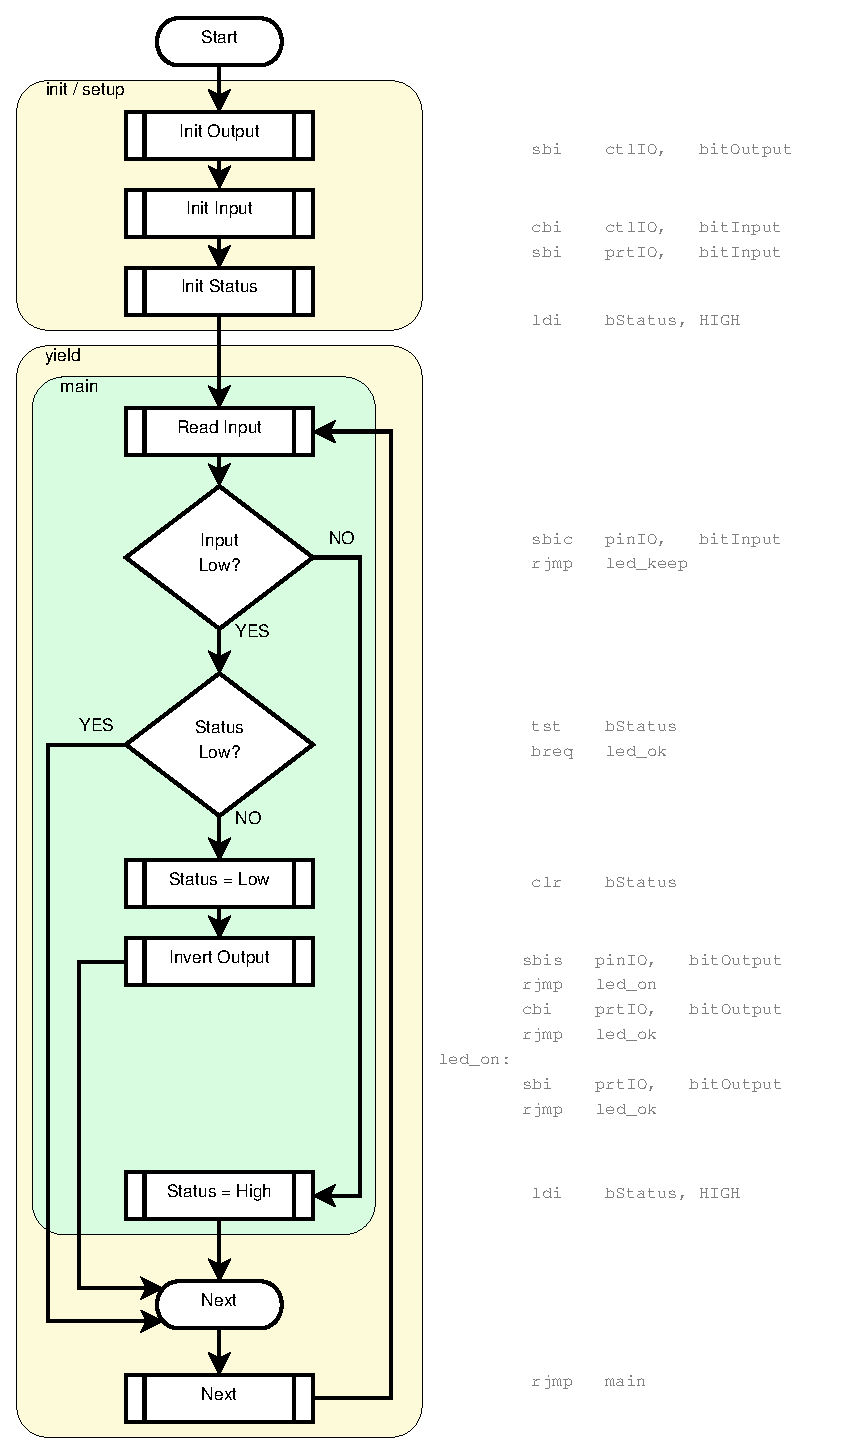
\includegraphics[height=0.95\textheight]{LED/S005_stable-decisions+symbols.eps}
!en   \caption{Stable Decisions - Flow Diagram}
!de   \caption{Stabile Entscheidungen - Ablaufplan}
  \label{S005FlowDiagam}
\end{figure}



!en X

!de Der grösster Störfaktor in der Informatik ist bekanntlich der Anwender. Nicht nur, dass seine Erwartungen von den Konzepten der Entwickler abweichen, es beginnt schon damit, dass er, in seinem Aufbau als Bioeinheit, unvorstellbar langsam ist. Die unglaubliche Langsamkeit des Anwenders ist ein technisches Problem, die Erwartungshaltung an die Art wie Geräte funktionieren ein ökonomisches. Wenn der gemeine Anwender unser Gerät nicht akzeptiert, wird er es nicht kaufen und wir haben nichts zu essen.



!en \subsubsection{Slow users}
!de \subsubsection{Die unglaubliche Langsamkeit des Anwenders}



!en X

!de Eine Bioeinheit drückt einen Knopf und unser Gerät hat zu reagieren. Dummer Weise prüft unser Gerät den Schalter vielleicht 1.000.000 Mal in jeder Sekunde. Ein Mensch z.B. mag einen Knopf sehr schnell drücken und den Kontakt im Schalter für 0.2s schliessen. Unser Gerät erkennt während dessen 200.000 Mal, dass der Schalter durchgeschaltet ist. Dies wohlgemerkt bei einem ganz schnellen Menschen. Was der Mensch aber erwartet ist:

\begin{center}\textit{
!en Change the light ones as I press (in my view) the button ones!
!de Schalte das Licht einmal um wenn ich (aus meiner Sicht) den Knopf einmal drücke. 
\end{center}}



!en X

!de Das Gerät darf also nur einmal umschalten auch wenn es 200.000 Mal feststellt, dass der Knopf gedrückt ist. Aus diesem Grund halten wir uns am Wechsel des Schaltzustandes fest um den Vorgang des Schaltens zu erkennen. Wir müssen also erkennen, ob sich der Zustand am Eingangbein unseres Microcontrollers \textit{geändert} hat! Dazu benötigen wir einen Zwischenspeicher, der den Schaltzustand bei der vorherigen Messung speichert. Wechselt dieser Zustand, müssen wir das Licht umschalten.



!en \subsubsection{Flickering}
!de \subsubsection{Prellen}



!en X

!de Problematisch dabei ist, dass elektrische Schalter prellen. Das heisst, sie stellen den Kontakt nicht so her wie wir es annehmen. Anstatt einmal einzuschalten, prallen die mechanischen Elemente des Schalters beim Aufprall voneinander ab und trennen die Verbindung wieder, um sie Millisekunden später dank der Elastizität der Schaltelemente wieder zu schliessen. Das kann sich unterschiedlich oft wiederholen. Wie das genau abläuft ist von unzähligen Faktoren abhängig. Die elektrische Konsequenz ist vereinfacht in Grafik \ref{S005SignalDiagam-Flicker} dargestellt.



!en X

!de Diesem Problem begegnen wir elektronisch. Anstatt mit dem Schalter einfach direkt das Bein des Eingangs am Schaltkreis auf Masse zu ziehen, verzögern wir die Spannungsänderung mit einem Kondensator wie in Abbildung \ref{S005FlickerReduction}.


%\begin{wrapfigure}{R}{0.25\textwidth}
\begin{figure}[htbp]
  \centering
%  \begin{center}
    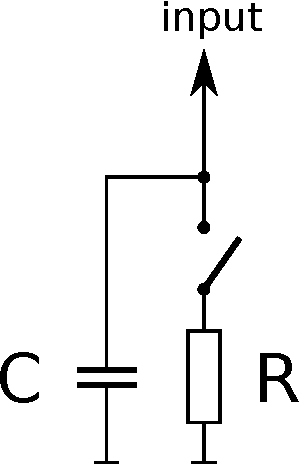
\includegraphics[width=0.24\textwidth]{LED/S005_stable-decisions_no-flicker.pdf}
%  \end{center}
!en   \caption{Flicker reduction}
!de   \caption{Prellunterdrückung}
  \label{S005FlickerReduction}
\end{figure}




!en X

!de Die Auswirkung dieser Massnahmen wird in Abbildung \ref{S005SignalDiagam} dargestellt. Grafik \ref{S005SignalDiagam-Ideal} zeigt den Spannungsverlauf am Eingangsbein des Microcontrollers wie wir ihn uns wünschen. In der Grafik \ref{S005SignalDiagam-Ideal+C} kann man erkennen, wie sich das Hinzufügen eines Kondensators (und des Widerstandes) darauf auswirken würde. Beim idealen rechteckigen Spannungsverlauf, wäre der Umschaltzeitpunkt identisch mit dem Zeitpunkt des Signalwechsels am Eingang des Microcontrollers. Durch den Kondensator wird dieser Umschaltzeitpunkt verzögert.




!en X

!de Den vereinfachten tatsächlichen Spannungsverlauf beim Schalten des Schalters zeigt Grafik \ref{S005SignalDiagam-Flicker} während Grafik \ref{S005SignalDiagam-Flicker+C} demonstriert, auf welche Weise uns der Einsatz eines Kondensators, der über einen Widerstand geladen wird, vor unkontrollierten Signalen schützt.




!en X

!de Die Kreise '\texttt{a}' und '\texttt{b}' umkreisen die Punkte an denen der tatsächliche Spannungsverlauf die Umschaltschwellen von \texttt{1} nach \texttt{0} (bzw. umgekehrt) schneidet und am Microcontoller tatsächlich der Eingangspegel wechselt. Die vertikale rote Linie in den Grafiken \ref{S005SignalDiagam-Ideal+C} und \ref{S005SignalDiagam-Flicker+C} zeigen den Moment, ab dem unser Programm den Wechsel der Eingangsspannung feststellen kann.



\begin{figure}%[htbp]
  \begin{subfigure}[htbp]{0.485\textwidth}
    \centering
    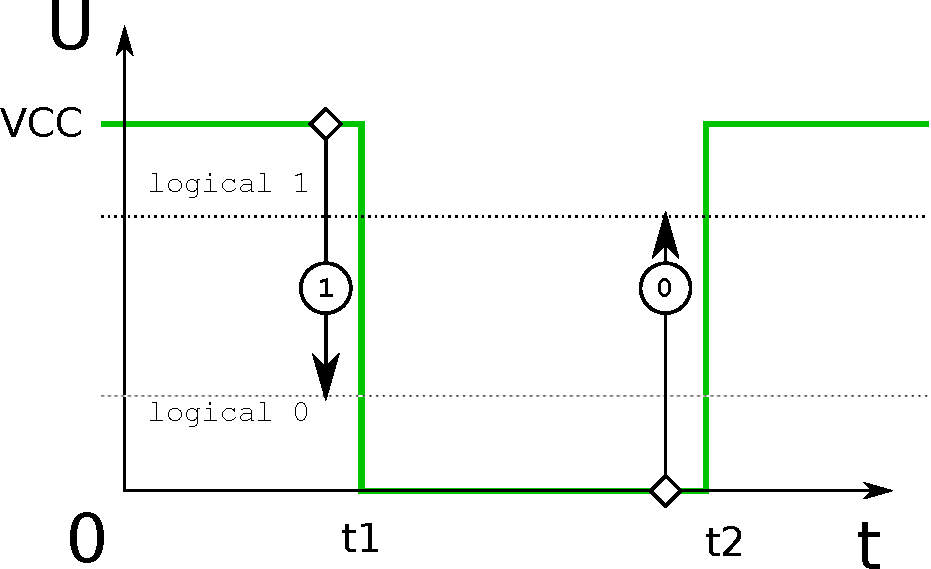
\includegraphics[width=\textwidth]{LED/S005_stable-decisions_ideal_signal.pdf}
    \caption{ideal}
    \label{S005SignalDiagam-Ideal}
  \end{subfigure}
  \quad
  \begin{subfigure}[htbp]{0.485\textwidth}
    \centering
    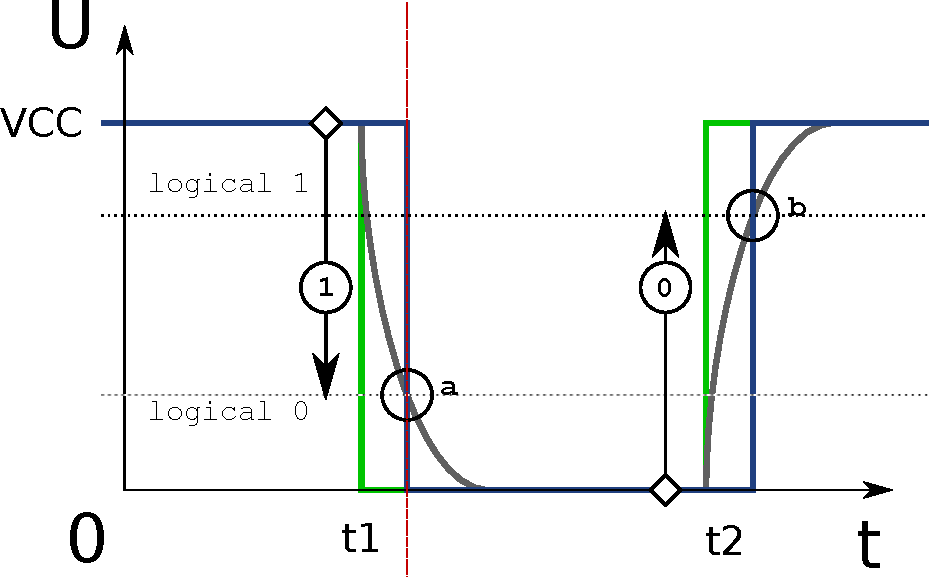
\includegraphics[width=\textwidth]{LED/S005_stable-decisions_ideal_signal+C.pdf}
!en     \caption{ideal + Capacitor}
!de     \caption{ideal + Kondensator}
    \label{S005SignalDiagam-Ideal+C}
  \end{subfigure}

  \begin{subfigure}[htbp]{0.485\textwidth}
    \centering
    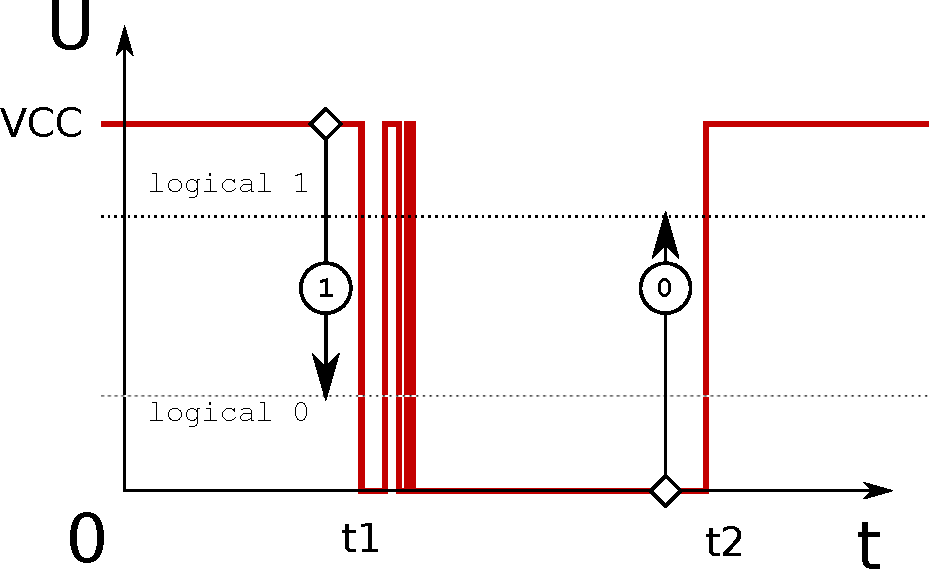
\includegraphics[width=\textwidth]{LED/S005_stable-decisions_ideal_signal+flicker.pdf}
!en     \caption{flickering}
!de     \caption{prellend}
    \label{S005SignalDiagam-Flicker}
  \end{subfigure}
  \quad
  \begin{subfigure}[htbp]{0.485\textwidth}
    \centering
    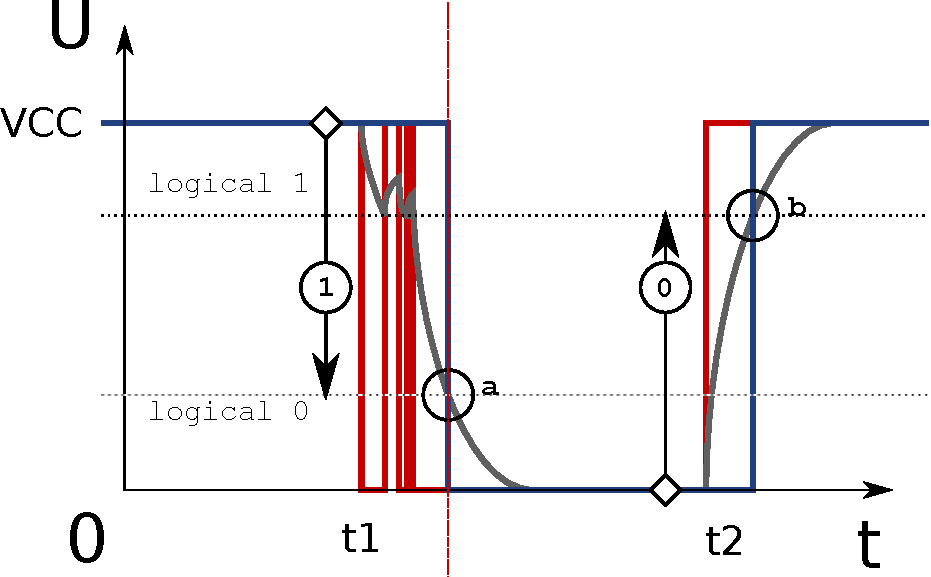
\includegraphics[width=\textwidth]{LED/S005_stable-decisions_ideal_signal+flicker+C.pdf}
!en     \caption{flickering + Capacitor}
!de     \caption{prellend + Kondensator}
    \label{S005SignalDiagam-Flicker+C}
  \end{subfigure}
!en   \caption{Stable Decisions - Signal Diagram}
!de   \caption{Stabile Entscheidungen - Signaldiagramme}
  \label{S005SignalDiagam}
\end{figure}

%\begin{figure}[htbp]
%  \centering
%  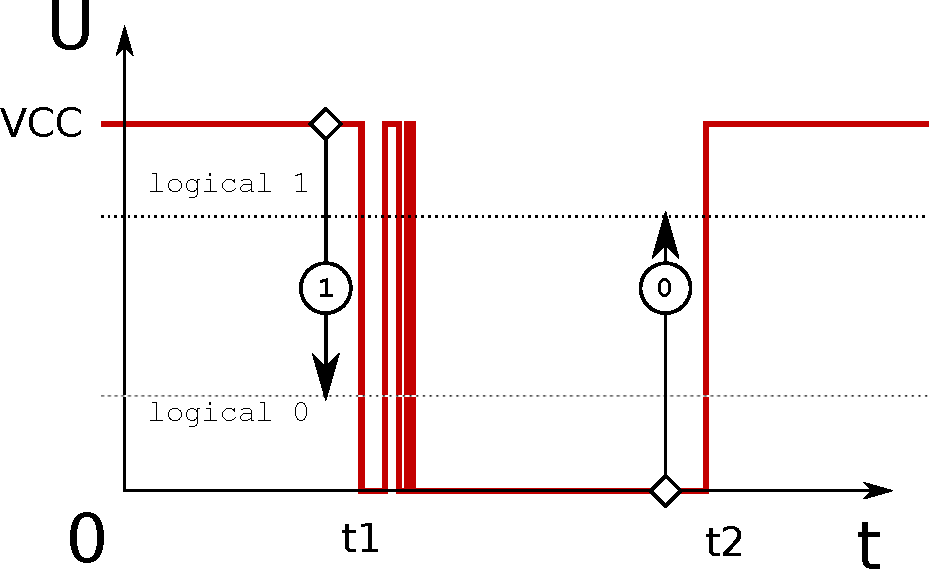
\includegraphics[width=80mm]{LED/S005_stable-decisions_ideal_signal+flicker.pdf}
%  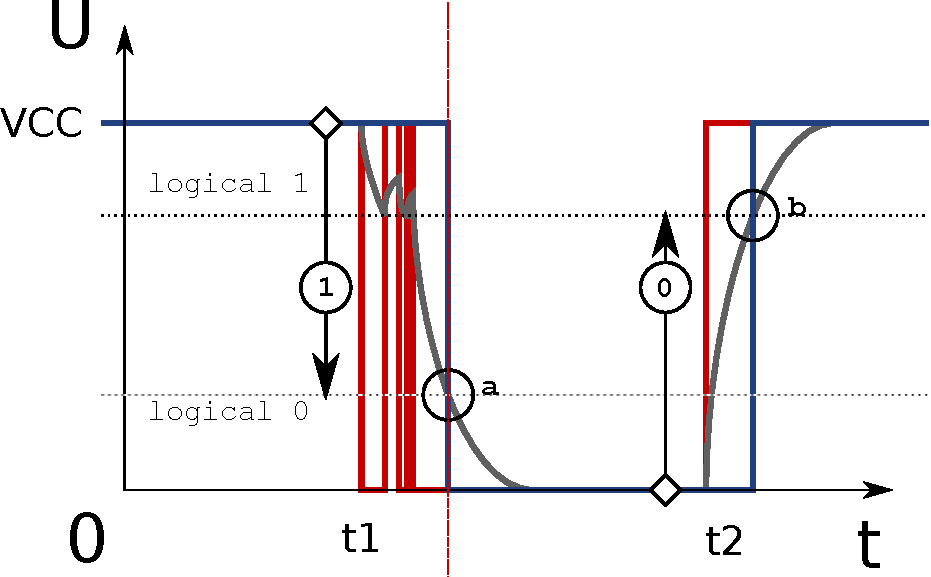
\includegraphics[width=80mm]{LED/S005_stable-decisions_ideal_signal+flicker+C.pdf}
%!en   \caption{Stable Decisions - Signal Diagram flickering without and with Capacitor}
%!de   \caption{Stabile Entscheidungen - Signaldiagramm prellend ohne und mit Kondensator}
%  \label{S005SignalDiagam-ideal+flicker+C}
%\end{figure}



!en X

!de Die blaue Linie in Grafik \ref{S005SignalDiagam-Flicker+C} zeigt den Verlauf des Pegels am Eingang nach dem Bedienen des Schalters, dessen Folgen in der roten Linie zu sehen sind. Man könnte den Eindruck gewinnen, als träte infolge der Kondensatorschaltung eine nennenswerte Schaltverzögerung ein. Dies ist aber nicht der Fall. Die Verzögerung liegt, je nach Dimensionierung des Kondensators und des Widerstandes im Bereich von Microsekunden oder Millisekunden. Eine Verzögerung also, die also nur für Maschinen spürbar ist. Die Grafiken in Abbildung \ref{S005SignalDiagam} täuschen über die wahren Verhältnisse hinweg.



!en \subsubsection{Fast feedback}
!de \subsubsection{Schnelle Rückmeldung}



!en X

!de Unser einziges Rückmeldegerät, mit dem wir dem Anwender unserer Applikation auch nur irgend etwas anzeigen können ist die angesteuerte Lampe/LED. Es gibt sonst nichts. Darum bleibt uns als Kommunikationsschnittstelle nur die angesteuerte Lichtquelle selbst. Auch wenn es in manchen Filmen cool erscheinen mag, wenn Akteure ohne Rückmeldungen an komplizierten Anlagen herumspielen und irgendwo in der Welt passiert etwas, die normale Bioeinheit erwartet eine 'sofortige Reaktion' für jede erfolgreiches Aktion. Passiert das nicht, wird es für den Nutzer schwierig.



!en X

!de Wie bereits erwähnt, zwingt uns diese Erwartungshaltung dazu, auf das Auftreten der ersten Schaltflanke im Schaltzyklus (HOCH nach NIEDRIG oder \texttt{1} nach \texttt{0}) zu reagieren. Wir kümmern uns nur um den Moment, in dem der Eingangspegel abfällt. Das ermöglicht uns auf die beiden wichtigen Aufgaben zu reagieren die vor uns stehen.

\begin{itemize}
!en   \item Give feedback as fast as possible
!de   \item So schnell wie möglich Rückmeldung geben
!en   \item Switch only ones if the user switches (in his eyes) ones
!de   \item Nur einmal schalten wenn der Nutzer glaubt, nur einmal geschaltet zu haben
\end{itemize}



!en \subsection{Finding the event}
!de \subsection{Das richtige Ereignis finden}



!en X

!de Für den Microcontroller erscheint alles was Menschen tun und erleben regelrecht endlos langwierig. Einmal ist der Schalter für Millionen Arbeitszyklen gedrückt, dann wieder für Milliarden von Zyklen losgelassen. In all dieser endlosen Langeweile passiert manchmal etwas. Um unseren Moment zu finden, muss unser Programm feststellen, dass sich etwas geändert hat.



!en X

!de Änderungen können nur im Vergleich zwischen zwei Zuständen festgestellt werden! Messen können wir zur gleichen Zeit aber nur einen Zustand. Das heisst, unser Programm muss sich merken, wie der Zustand bei der letzten Messung war um diesen mit der aktuellen Messung zu vergleichen.



!en X

!de War der Zustand eben noch HOCH und wurde in der Aktuellen Messung als NIEDRIG festgestellt ist das lang ersehnte Ereignis eingetreten. Dann muss das Programm handeln, also den Schaltzustand der LED umkehren.



!en \subsection{And some modesty}
!de \subsection{Programmierte Umsicht}


!en X

!de In Rücksichtnahme auf die Dinge, die noch kommen werden, müssen wir Umsicht walten lassen. Die Endlosschleife, die unser Programm am Leben und um Zaum hält, führt (ganz allgemein) einige wichtige Aufgaben aus:

\begin{itemize}
!en   \item It mostly contains the main program
!de   \item Sie enthält den grössten Teil des Hauptprogramms
!en   \item It possibly consist of multiple parts
!de   \item Dieses Programm besteht vielleicht aus mehreren Teilen
!en   \item It consist of an undefined amount of functional separate program parts
!de   \item Wenn es Teile gibt, haben diese völlig verschiedenen Aufgaben
\end{itemize}



!en X

!de Darum müssen wir darauf achten, dass wir keine voreiligen Schlüsse ziehen und Programmteile überspringen, in der Annahme dass darin nichts mehr passieren würde. Ebenso wie es nur einen Highlander geben kann, kann es nur einen Sprung zurück zu '\texttt{main}' geben. Dieser Sprung befindet sich am Ende aller Funktionsbläcke in der Hauptprogrammschleife:

\begin{lstlisting}
main:

  A_begin:
            block     A or goto to end of block A
  A_end:

  B_begin:
            block     B or goto to end of block B
  B_end:

  C_begin:
            block     C or goto to end of block C
  C_end:

mein_end:
            finalise
            rjmp      main
\end{lstlisting}



!en X

!de Um konsistent zu bleiben, ist es ausserdem wichtig, dass einzelne Funktionsblöcke in sich geschlossen sind. Wir springen nicht von Block A nach Block B, sondern von Block A nach 'Ende von Block A'. Auf diese Weise bleiben die Blöcke unabhängig in können in ihrer Reihenfolge vertauscht werden ohne Gefahr zu laufen, den prinzipiellen Ablauf zu zerstören. Ein Block folgt dem nächsten und jeder Block ist unabhängig von jedem anderen Block.

\section{Stable Decisions Triggered}

If you feel a bit uncertain about our solution or if you have the feeling that all this should be done better you may be right. We would not ensure you that the following solution is better under every circumstance, but for some application, there is a much better way.

For this way we need to introduce the concept of interrupts.

The magic behind interrupts in micro controllers is much more as in simple CPUs!

Interrupts are special mechanics in processing units to enable the execution of code at a certain time or after a certain event by interrupting the normal processing, doing something else and after this continue whatever was interrupted.

In micro processors this mechanic is much more sophisticated. In micro controllers you may interrupt the system from nothing! Meaning, it is possible to nearly shut off the whole system, interrupt it from his deep sleep, let it do something and send it back to sleep again.

Such applications are useful if energy resources are small. For example, if you wish to drive your weather station one year on a single AAA cell or less, possibly supported by solar power.

In such applications you wish to reduce power consumption of your system as far as possible. There is no need to let your micro controller do eight million cycles per second if you take a measurement every ten minutes! It may be much better so stop the whole system until the next measurement is to start.

You already may expect it. Such code does not need to loop with full processing power to do nothing, such code really does nothing while waiting:

\begin{lstlisting}
; LED/S005_stable-decisions-trigger.asm

.DEVICE atmega8

.org 0x0000
            rjmp    start
            rjmp    trigger0
            
start:
            ...
            
main:
            sleep
            rjmp    main

trigger0:
            do_it
            reti
\end{lstlisting}

This approach also has the advantage to don't need the otherwise necessary status accumulator register and consequently no comparison between former and current status. It simple needs to change the current status of the light if called.

!en \section{Light Shift}
!de \section{Lichtverschiebung}

!en X

!de Langsam wird es Zeit etwas anzugeben. Nur ein wenig! Wir werden drei LEDs in eine Reihe schalten und eine nach der anderen einschalten. Der Wechsel wird jeweils mit einem Druck auf den Schalter ausgelöst.



!en It would be much easier to do this with 8 lights, but here we are. We will keep the existing circuit as untouched as possible and, not at last, we are constantly on he search for a challenge.

!de Es wäre viel einfacher, das mit 8 LEDs zu machen, dafür haben wir aber zu wenig Platz. Wir werden die existierenden Schaltung weitgehend unberührt lassen und nur die LEDs hinzufügen.


!en X:

!de Dies ist der erweiterte Schaltplan, die Erweiterung ist, wie gewohnt, rot gekennzeichnet.

\begin{figure}[htbp]
  \centering
  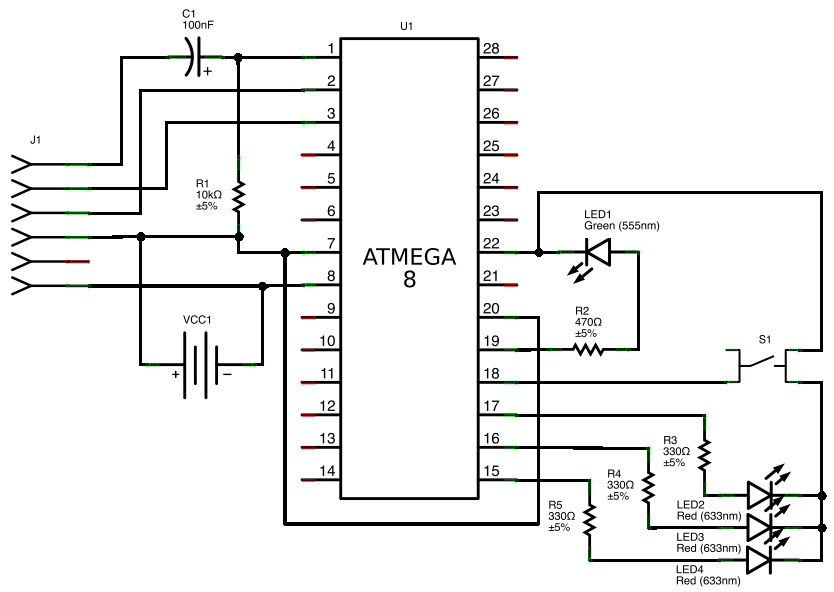
\includegraphics[width=120mm]{LED/S010_light-shift_Circuit_schema.png}
!en   \caption{Light Shift - Schema}
!de   \caption{Lichtverschiebung - Schaltplan}
  \label{atmega8-light-shift-schema}
\end{figure}



!en X

!de Die zusätzlichen LEDs haben wir direkt hinter die bereits vorhandene LED angeschlossen. Das ist am einfachsten auf dem Breadboard führt aber leide rzu einer erhöhten Komplexität des Programmcodes:

\begin{lstlisting}
; LED/S010_light-shift.asm

.DEVICE atmega8


.equ ctlIO         = DDRB
.equ prtIO         = PORTB
.equ pinIO         = PINB

.equ bitSignal     = 5
.equ bitInput      = 4
.equ bitLightStart = 3

.equ mskLightShift = 0x0E

.equ LOW           = 0
.equ HIGH          = 1

.def bStatus       = r16
.def bTemp         = r17
.def bData         = r18


.org 0x0000
            rjmp    start


start:
            ldi     bTemp,        mskLightShift | 1 << bitSignal
            out     ctlIO,        bTemp
            ldi     bTemp,        1 << bitInput | 1 << bitSignal
            out     prtIO,        bTemp

            ldi     bStatus,      HIGH

main:
            sbic    pinIO,        bitInput
            rjmp    led_keep
            tst     bStatus
            breq    led_ok
            clr     bStatus

            in      bData,        pinIO
            mov     bTemp,        bData
            andi    bData,        0xFF - mskLightShift
            ori     bData,        1 << bitInput

            andi    bTemp,        mskLightShift
            lsr     bTemp
            andi    bTemp,        mskLightShift
            brne    shift_ok
            ldi     bTemp,        1 << bitLightStart
shift_ok:
            or      bData,        bTemp
            out     prtIO,        bData

            rjmp    led_ok
led_keep:
            ldi     bStatus,      HIGH
led_ok:
            rjmp    main
\end{lstlisting}

As you can see, we have some changes to the former code. This is, in the hole, because we have to deal with four instead of one lights. One light (the one we toggled last time) will serve as signal light. It is lighting up after our micro controller has finished booting. The other three LEDs will be used to shift the light. In our case this means we start off with one of the three lights ON and each time we press our button the next light lights up whilst the former light shuts off.

Our code reflects the higher complexity at the first look with more constants and more named registers. Already we are using 10\% of all available registers and 20\% of all registers usable for generic purpose. This is bad news! Hopefully our resource consumption will not grow with constant speed.

Names for constants (not resources) we need besides the ones from the former sample are

\begin{lstlisting}
.equ bitLightStart = 3     ; as in  0b00001000

.equ mskLightShift = 0x0E  ; builds 0b00001110
\end{lstlisting}

\texttt{bitLightStart} is the number of the pin on the output port where the LED light of our light chain resides. A bit will be shifted this time to the left. The other LEDs are expected to use the two lower pins (2 and 1). Pin B0 on the \at can be found on the other side of the chips, so for our physical breadboard circuit it's a bit too far away to use it.

Please remember, such decisions are no fun. In reality you may sometimes be driven to compensate in software for simplification of hardware as PCB layout, different chip pinouts and so on. So we accept this situation as example of what may happen in real life.

\texttt{mskLightShift} is a bit mask containing bits at all pins of the output port where our light chain is connected to. We need such a bit mask because we need to shift the 'LED ON' bit around but won't shift any other bits found in the port data. So we use this bit mask to

\begin{itemize}
  \item mask out the relevant light chain bits from the rest
  \item mask out a too far shifted 'LED ON' bit (logical overflow)
  \item mask out the light chain bits in input data after querying our PORT
\end{itemize}


Named registers (resources) we need in addition to the former program are:
 
\begin{lstlisting}
.def bTemp         = r17
.def bData         = r18
\end{lstlisting}

\texttt{bTemp} will be used to shift our 'LED ON' bit around but \texttt{bData} has to give us the 'big picture' about our ports status. First before, second after shifting the 'LED ON' bit.

We start, as usual, by initialising the micro controller where it needs to be initialised. This time, we need to set all pins on our port the same time because the alternative is (for the moment) much too expensive. So we build a bit mask to send it to our IO ports data direction register (DDR):

\texttt{mskLightShift} combined with \texttt{1 << bitSignal} makes \texttt{0b00101110}. Sending this byte to DDRx will set pins 1, 2, 3, 5 to output and all other pins to input mode.

\begin{lstlisting}
start:
            ldi     bTemp,        mskLightShift | 1 << bitSignal
            out     ctlIO,        bTemp
            ldi     bTemp,        1 << bitInput | 1 << bitSignal
            out     prtIO,        bTemp
\end{lstlisting}

Then we need to do three things by sending a byte to PORTx:

\begin{itemize}
  \item Switch ON LED on pin 5 (\texttt{bitSignal})
  \item Set pin 4, our input pin, to 'pulled up' (\texttt{bitInput})
  \item Set all other pins to off/offline
\end{itemize}

All this is done by mixing all active bits together and sending the mix \texttt{(0b00110000)} to the port. After doing so the signal LED is on, the light chain is off. Until \texttt{clr bStatus} nothings more has changed. Also the rest with and after label \texttt{led\_keep} is kept the same.

The changed part is this:

\begin{lstlisting}
            in      bData,        pinIO
            mov     bTemp,        bData
            andi    bData,        0xFF - mskLightShift
            ori     bData,        1 << bitInput

            andi    bTemp,        mskLightShift
            lsr     bTemp
            andi    bTemp,        mskLightShift
            brne    shift_ok
            ldi     bTemp,        1 << bitLightStart
shift_ok:
            or      bData,        bTemp
            out     prtIO,        bData
\end{lstlisting}

All magic resides in these lines. It's not too much, so we simply explain it sequentially.

We need to get the ports state and unfortunately we have to understand more about this than is good for the program. We have to send back the whole data byte, modified only in the part where the LED chain state changed. BUT (!) we also need to ensure, our input pin keeps his pull up resistor active. Otherwise we loos our connection to the outer world!

Next we need to split the read byte/data in two parts. The one containing constant data and the other one containing the bits to be shifted.

Phase one therefore copies \texttt{bData} to \texttt{bTemp}, then masks out all bits dealt with in the bit shifting process and finally adding/regenerating the 'pull up' bit for port \texttt{bitInput}.

Phase two masks out all bits not related to the bis shifting operation, shifts the remaining bit and masks the result again with the same mask. If this operation leads to a result of ZERO/EQ/NULL, then we have shifted out our bit and need to insert a new one at the start position inside the byte where the bit starts its decent, at: \texttt{bitLightStart}.

Phase three then combines our static bits with our manipulated one and output all together to our combined input/output port.



\chapter{Time}

\section{Instable Elements}

The longest time we tried to avoid the simplest demo in most Arduino beginners sets. The blinking light demo! Some of our readers may have ask themselves where the problem should be. Now is the moment to explain.

We do not want to make a fuss with code we would have to be ashamed of but couldn't bring us to start with timers and interrupts before introducing the most basic principles of programming. Please remember, using assembler language brings us in a position of power which forces us into reliability.

There is no way a reliable programmer would use 4.000.000 NOPs ('no operation' operations) twice to let a light blink ones per second. Also, we hope, no one reading until this point would keep it as responsible to enter a loop, busying our poor micro controller to wait half a second by wasting four million CPU cycles.

So we had to experiment enough to enter the reign of timers and interrupts. Staying our ground not demonstrating bad code, keeping the book pure, we don't show only a part of a single bad example in code. You may remember it in your dreams!

To cut a long story short. Here its the code:

\begin{lstlisting}
; LED/S020_instable-elements.asm

.DEVICE atmega8

.org 0x0000
            rjmp    start 

start:
            ...            
main:
            rjmp    main
\end{lstlisting}



\part{External devices}

\chapter{Shift Registers}

\section{SRAM to Shift Register}

Sending SRAM content/data to shift registers has some applications. Some of them are

\begin{itemize}
  \item {Light chains}
  \item {Raster displays}
\end{itemize}

It is an important way to communicate with the technical environment in certain situations. Most importantly if you have more bit to output as pins on your micro controller.


\part{How to start}

\chapter{Hardware & Setup}

\section{Minimal hardware setup}

In this section the minimal hardware setup to get your AVR up and running. You will need the following things for a very basic setup

\begin{itemize}
  \item {1x 5V power supply}
  \item {1x Solderless breadboard}
  \item {1x AVR IC (we will use the ATmega8)}
  \item {some jumper wire}
  \item {1x ISP programmer}
\end{itemize}




\end{document}
